
\onecolumngrid

\section*{Supplementary material}

This supplementary material provides evidence supporting the methods and arguments in the main text, including empirical mitigation of lattice artifacts, comparisons among lattice groups, comparisons between lattice and phenomenology, and uncertainty estimates. 

\begin{figure}
    \centering
    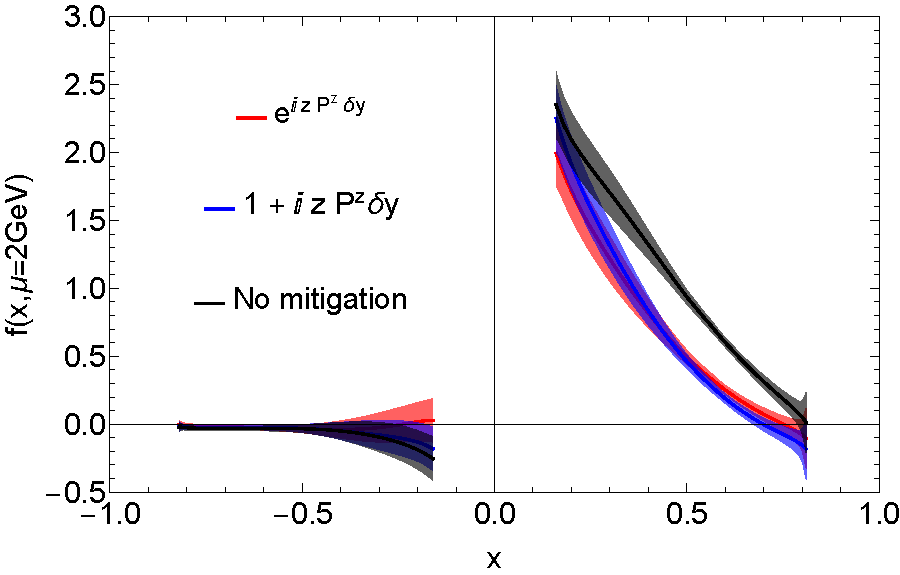
\includegraphics[width=0.5\linewidth]{./figs/f_MSU20_compareforms.pdf}
    \caption{Proton's unpolarized isovector PDFs calculated using different forms to mitigate lattice artifacts. The dataset is the MSULat20~\cite{Lin:2020fsj} extrapolated to the physical limit. The red band is related to the exponential mitigation form adopted in the main context. The blue band corresponds to the linear correction form. The black band represents the result without mitigation. }
    \label{fig:f_MSU20_compareforms}
\end{figure}
Fig.~\ref{fig:f_MSU20_compareforms} tests whether the PDF results are sensitive to the choice of correction forms to mitigate lattice artifacts. The red band shows the PDF result related to the exponential form in Eq.~(\ref{eq:CalM}) of the main text, $e^{i z P^z \delta y}$. The blue band corresponds to the linear form $1 + i z P^z \delta y$. The two results are consistent within uncertainties, indicating that the resulting PDFs are not strongly sensitive to the two correction forms considered here. For reference, the black band does not mitigate the lattice artifacts and deviates from the others, indicating the importance of removing genuine lattice artifacts.  

\begin{figure}
    \centering
    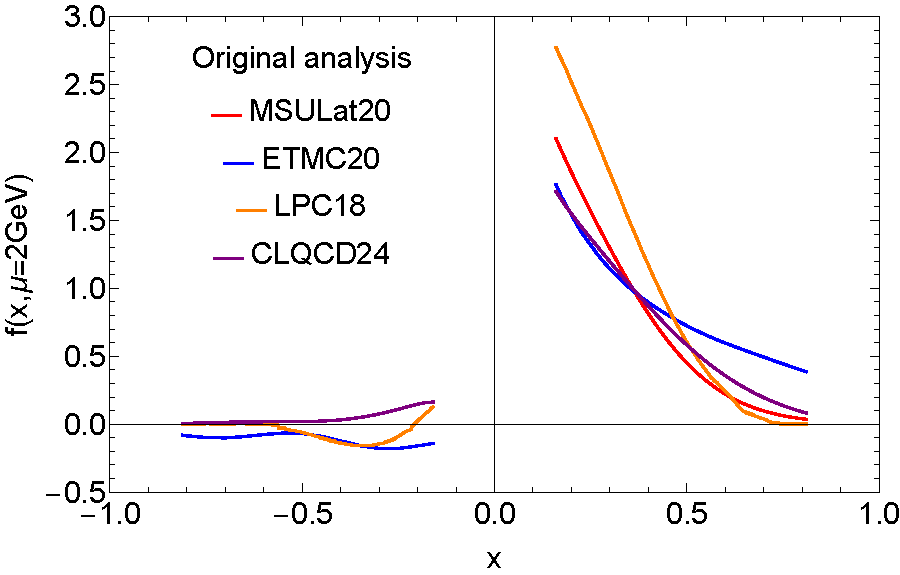
\includegraphics[width=0.48\linewidth]{./figs/f_before.pdf}
    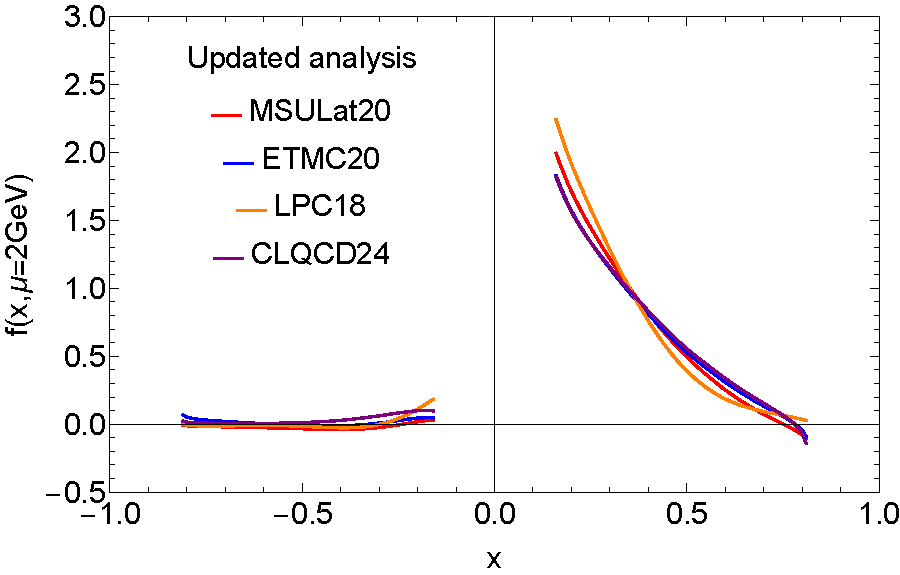
\includegraphics[width=0.48\linewidth]{./figs/f_after.pdf}
    \caption{Comparison between the analysis in the original literature~\cite{Lin:2020fsj,Alexandrou:2020qtt,LatticeParton:2018gjr,Chen:2024rgi} (left panel) and the reanalysis in this work (right panel). Only the central values are displayed. The spread across different lattice groups is reduced under the updated analysis.}
    \label{fig:f_before_after}
\end{figure}
Fig.~\ref{fig:f_before_after} compares the resulting lattice PDFs before and after the reanalysis. The left panel corresponds to the original analysis in Refs.~\cite{Lin:2020fsj,Alexandrou:2020qtt,LatticeParton:2018gjr,Chen:2024rgi}. The red, blue, and orange curves are digitized from the relevant plots in Refs.~\cite{Lin:2020fsj,Alexandrou:2020qtt,LatticeParton:2018gjr}, respectively. Since Ref.~\cite{Chen:2024rgi} does not directly display the $u-d$ combination, we calculate the purple curve using the data and methods in Ref.~\cite{Chen:2024rgi}. The right panel shows the updated analysis in this work, for which the spread among the lattice datasets is substantially reduced.   

\begin{figure}
    \centering
    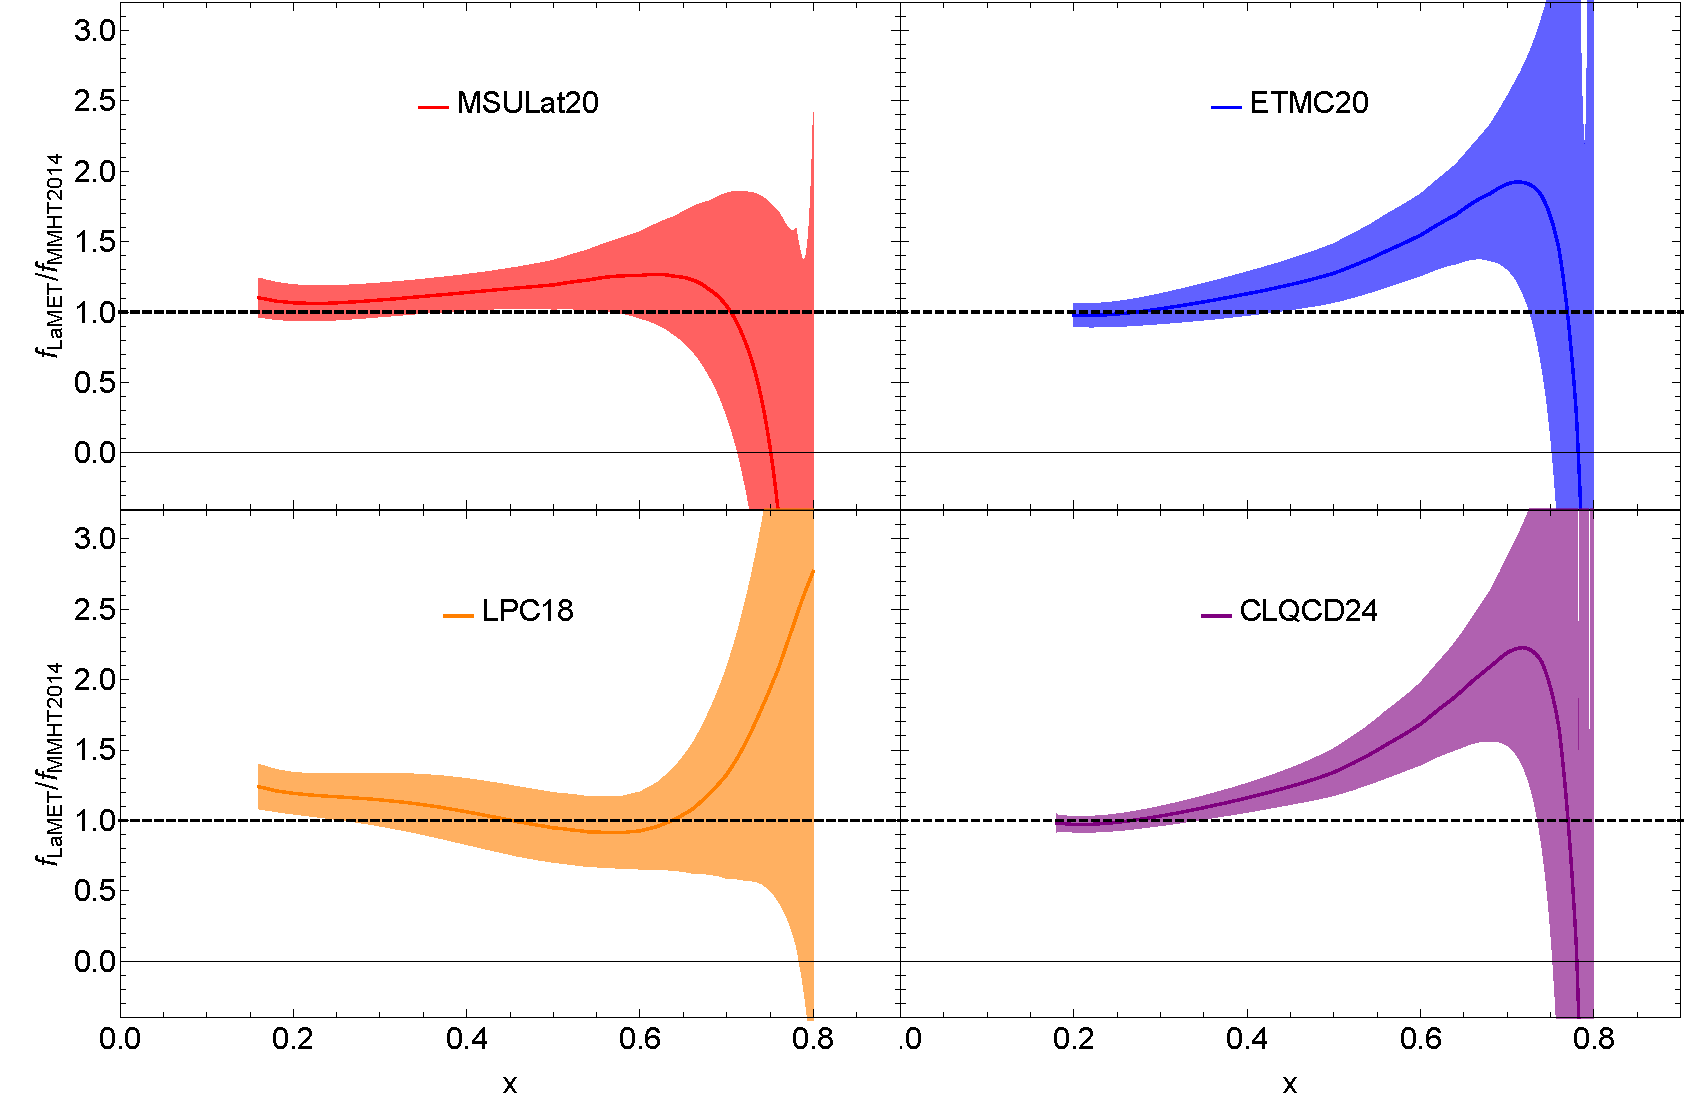
\includegraphics[width=0.8\linewidth]{./figs/f_ratio.pdf}
    \caption{The ratios between PDFs from LaMET and MMHT2014~\cite{Harland-Lang:2014zoa}. }
    \label{fig:f_ratio}
\end{figure}
To better compare LaMET and global fit PDFs, we plot their ratios in Fig.~\ref{fig:f_ratio}. The LaMET result from the physical-limit dataset, MSULat20, shows $\sim 1 \sigma$ agreement with the global fit PDF. The other datasets are broadly compatible with the global fit, with residual deviations that may arise from discretization or unphysical pion-mass effects. 

\begin{figure}
    \centering
    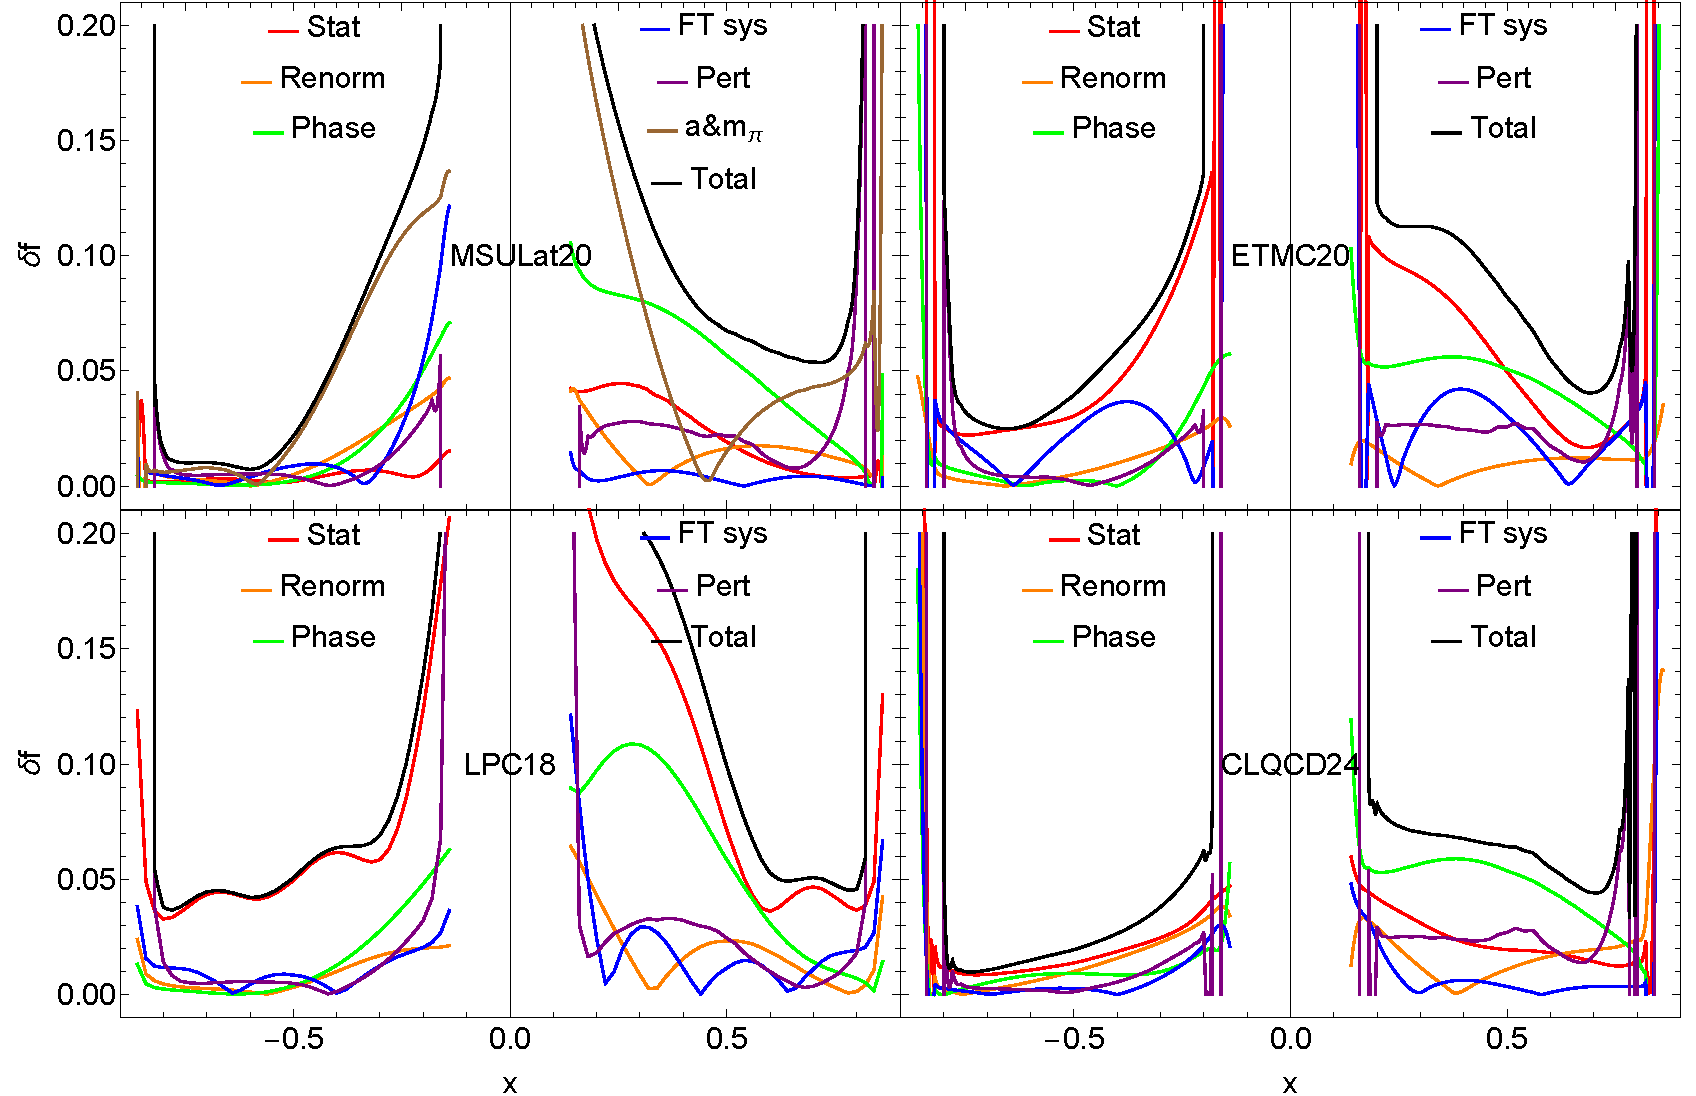
\includegraphics[width=0.8\linewidth]{./figs/f_err_all.pdf}
    \caption{Uncertainties for proton's unpolarized isovector PDFs in Fig.~\ref{fig:lcPDF}. The red curve is the statistical uncertainty. The orange curve arises from the uncertainty of $m_0$ in the renormalization. The green curve is the uncertainty from the phase rotation parameter $\delta y$. The blue curve is the systematic uncertainty of the Fourier transform estimated as the difference between LA and NLA. The purple curve denotes the uncertainty of perturbative matching evaluated through the variations of physical scales in the RG evolution studied in Ref.~\cite{Ji:2024hit}. The brown curve is the systematics from the continuum and physical pion mass extrapolations, estimated using the deviation among various ansätze in Fig.~4 of Ref.~\cite{Lin:2020fsj}. The black curve is the total uncertainty obtained by treating the individual contributions as uncorrelated and adding them in quadrature. }
    \label{fig:f_err_all}
\end{figure}
Fig.~\ref{fig:f_err_all} shows the detailed uncertainty estimates. The red curves correspond to statistical uncertainties $\sigma_{\rm stat}$, with ETMC20, LPC18, and CLQCD24 calculated using bootstraps, which automatically take into account data at $|z|<z_L$ and the extrapolated form at $|z|>z_L$, as well as their correlations. For MSULat20, we combine in quadrature the statistical uncertainties digitized from Fig.~5 in Ref.~\cite{Lin:2020fsj} with those propagated from the fitted large-distance forms. We find that the former source of statistical uncertainty is much larger than the latter, e.g., 0.019 vs. 0.003 at $x=0.5$, indicating that the uncorrelated combination of the two sources~\footnote{The correlation within each source is considered.} will not deviate much from the correlated one. The orange curves $\sigma_{\rm renorm}$ arise from the uncertainty of $m_0$ in the renormalization. Since $m_0$ is determined by fitting the perturbative Wilson coefficients, the perturbative uncertainties are propagated into $m_0$, which eventually affects the momentum-space PDFs. The green curves $\sigma_{\rm phase}$ come from the uncertainties of $\delta y$ in the mitigation form, which originate from the first moment~\cite{Djukanovic:2024krw}, $\langle x \rangle(\mu=2\, {\rm GeV})=0.153(17)$. The blue curves $\sigma_{\rm FT \, sys}$ are the systematic uncertainties of the Fourier transform, estimated as the difference between LA and NLA, following the method in Ref.~\cite{Ji:2026vir}. The purple curves $\sigma_{\rm pert}$ originate from perturbative matching uncertainties, estimated by varying the physical scales in the RG evolution following Ref.~\cite{Ji:2024hit}. The brown curve $\sigma_{a\& m_{\pi}}$ for MSULat20 denotes the systematics from the physical extrapolations, estimated using the deviation among various ansatze in Fig.~4 of Ref.~\cite{Lin:2020fsj}. When we calculate the uncertainty for one step, the parameters at other steps are set to their central values. The total uncertainty $\sigma_{\rm tot}$ is obtained by treating these contributions as uncorrelated and adding them in quadrature,
\begin{align}
\sigma_{\rm tot} = \sqrt{ \sigma_{\rm stat}^2 + \sigma_{\rm renorm}^2 + \sigma_{\rm phase}^2 + \sigma_{\rm FT \, sys}^2 + \sigma_{\rm pert}^2 + \sigma_{a\& m_{\pi}}^2} \ ,
\end{align}
where $\sigma_{a\& m_{\pi}}$ is considered only for MSULat20 and not included for other datasets. 